%! Author = Saeid Yazdani
%! Date = 7/28/2024

\section{The Digital-Twin Approach}
\label{sec:digital-twin-approach}

For decades, we have utilized predictive controllers \autocite{holtzj}
and digital twin models \autocite{aivaliotis} which are based on a near-perfect
representation of real-world situations.

This model allows us to simulate the system's response to any external
influence.
By monitoring all states at any given time, we can predict the future behavior
of a signal chain at its output by measuring internal nodes.

Internal monitoring is crucial for accurately predicting system behavior,
especially in large systems with inherent delays.
In real-life scenarios, it takes a full round-trip delay to observe the output
behavior in response to an input change.
However, with a digital twin, we can calculate (predict) the output signal
much faster.

\subsection{Digital Control Loop with Internal Monitoring}
\label{subsec:digital-control-with-internal-monitoring}

Internal nodes provide insight into the future shape of the waveform if
correction values are not applied.
Utilizing the principles of digital twin methods, we monitor internal signal
waveforms at the early stages of signal flow and predict the output behavior
without corrections.
Based on these predictions, we generate correction signals to minimize unwanted
effects such as ringing or slow signal rise.

The downside of gaining better insight is the increased instrumentation effort,
requiring a balance between system speed, accuracy, and instrumentation costs.

Implementing \acs{FPGA}-based \acs{DSP} in all feedback loops offers maximum
flexibility to achieve the desired signal quality.
Replacing less critical local feedback loops with simple analog feedback
structures (hence the hybrid analog-digital approach) can help to reduce design
and production costs.

The differences between time-invariant and time-variant compensation require
that we evaluate the actual load conditions before generating any signal.
This involves several steps:

\begin{itemize}[topsep=8pt,itemsep=4pt,partopsep=4pt, parsep=4pt]

    \item
    \textbf{Small Signal Analysis:} We apply an infinitesimal signal and observe
    the system response to understand its behavior.

    \item \textbf{Predictive Modeling:} Based on the small signal analysis, we
    predict the system's behavior.
    This allows us to anticipate how the system will react to various
    inputs and conditions.

    \item \textbf{Dynamic Compensation Adjustment:} We initially apply the
    best-case compensation to achieve fast settling.
    During this process, we continuously monitor the system and dynamically
    adjust the compensation to ensure the optimal final settling.
    This means achieving the target response with minimal overshoot and the
    shortest time to enter the target channel.

\end{itemize}

Implementing this approach requires fast \acs{DSP} cores and high-speed
signal converters (\acs{ADC} and \ac{DAC}).
Fortunately, modern technology provides these components at a reasonable cost,
making digital-based compensation feasible.

\autoref{fig:internal-monitoring-structures} shows the necessary digital
structures and their typical delays to have full observance over the control
loop behavior of the proposed time-variant system at each critical stage
(\autoref{fig:system-block-diagram-hvs}).

\begin{figure}[p]
    \centering
    \vspace*{\fill}
    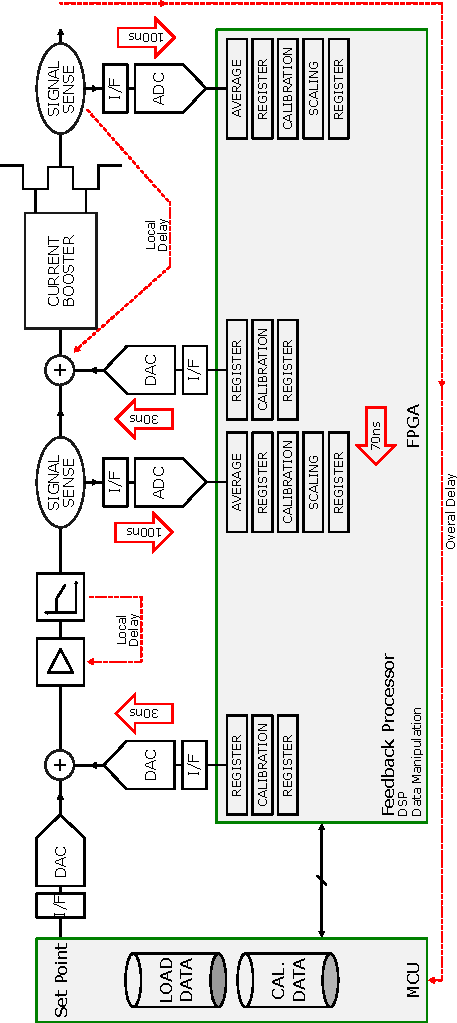
\includegraphics[
        width=\linewidth,
        height=0.86\textheight,
        keepaspectratio
    ]{figures/dps_algorithms_psu/internal_monitoring}
    \caption[Internal Monitoring Structures]{
        Arrays of a-to-d and d-to-a converters are necessary at critical
        stages of the proposed control system to enable full coverage over
        system response at each critical stage of the control loop.
        Typical expected delay values for digital components are denoted.
    }
    \label{fig:internal-monitoring-structures}
    \vspace*{\fill}
\end{figure}
